\documentclass[a4paper,11pt]{article}
\usepackage[utf8]{inputenc}
\usepackage[T1]{fontenc}
\usepackage[french]{babel}
\usepackage{amssymb}
\usepackage{enumitem}
\usepackage{graphicx}
\graphicspath{{imagesCR/}}
\usepackage{fancyhdr}
\usepackage{hyperref}
\usepackage[top=3cm,left=3cm,right=3cm,bottom=3cm]{geometry}
\renewcommand{\thesection}{\Alph{section}}
\begin{document}
\pagestyle{fancy}
\lhead{\textbf{Projet Picross}}
\rhead{\textbf{L2 Informatique}}
\title{PROJET PICROSS}
\author{KAJAK Rémi\\KINZY Érick\\MAROUF Taous\\NOUVELIÈRE Benjamin}
\date{\today}
\maketitle
\newpage
\tableofcontents
\listoffigures
\newpage
\section*{\LARGE I. \hspace*{0.1cm} Introduction}
\label{section*:introduction}
\addcontentsline{toc}{section}{I. \quad Introduction}
L’informatisation est le phénomène le plus important de notre époque. Elle s’immisce dans la plupart des objets de la vie courante, que ce soit dans l’objet proprement dit ou bien dans le processus de conception ou de fabrication de cet objet.\bigbreak
L’objet de notre travail est de programmer une version simplifiée du jeu \og Picross \fg{}, qui est un jeu de réflexion solitaire. Le but consiste à découvrir un dessin - ou un motif - sur une grille en noircissant des cases. Les valeurs données sur le côté gauche et en haut de la grille donnent des indices~: ils indiquent la taille des groupes de cases noires de la ligne ou de la colonne sur laquelle ils se trouvent. La difficulté est progressive, et au fur et à mesure de son avancée dans le jeu, le joueur doit résoudre des grilles comportant plus de cases et plus de groupes par rangée (ligne/colonne).\bigbreak
Notre objectif était de réaliser l’analyse et la conception d’un Picross en utilisant le langage C. Nous nous sommes servi des outils de base de la programmation, de la récursivité et avons manipulé des fichiers.\bigbreak
Dans ce rapport, nous allons tout d’abord exposer l’analyse de ce jeu, puis le codage et les méthodes utilisées.
\newpage
\section*{\LARGE II. Organisation du travail}
\addcontentsline{toc}{section}{II. \quad Organisation du travail}
\label{section*:organisation_travail}
Pour mener à bien la création du jeu avec le langage C, il a fallu trouver des structures et un moyen efficace pour stocker les données des puzzles à résoudre. Étant un jeu à grille, la définition et l'initialisation de matrices furent immédiatement envisagées. Quant au stockage des données, des fichiers texte possédant un format spécifique ont été créés pour répondre au besoin de la génération des données pour les matrices.
\section[Fonctions principales]{Découpe du problème en fonctions principales}
\label{section:fonctions_principales}
Pour ce faire, il a fallu définir quatre matrices principales avec une taille fixe~:\medbreak
\begin{itemize}[label=$\square$]
	\item une matrice solution où, pour un niveau donnée, le motif final serait présent~;
	\item deux matrices périphériques qui contiendraient les nombres des groupes, nécessaires à la résolution du puzzle par le joueur~;
	\item une matrice de jeu, vide par défaut, qui serait la grille de jeu pour l'utilisateur.
\end{itemize}\bigbreak
Différentes types de matrices ont été codées et testées - entre autre, une structure contenant une variable de type énumération -, mais au final, seules les matrices de type entier (utilisées pendant les tests unitaires) ont été préservées. La fonction la plus à même de remplir ce rôle est \textbf{init\_matrice([1 argument])}, où N est une constante pour la taille par défaut.\bigbreak
Les matrices ne suffisant pas pour le jeu, des fichiers texte ont été  conçus avec un format par défaut~:\medbreak
\begin{itemize}[label=$\square$]
	\item puzzles\_binaires.txt~;
	\item nombres\_puzzle.txt.
\end{itemize}\bigbreak
La fonction \textbf{lecture\_fic([5 arguments])} permet de lire ces fichiers et d'interpréter les données présentes. Le premier fichier texte contient des rangées de 0 et de 1 en clair qui sont directement assignées à la matrice solution~; les nombres des matrices périphériques sont générées ensuite avec la lecture de la première matrice. Quant au second fichier, il s'agit de l'opération inverse~: les nombres des matrices périphériques sont données, et il faut les utiliser pour générer la matrice solution.\bigbreak
Ces deux types de fichier sont nécessaires pour répondre aux deux parties demandées par la liste des sujets montrée au début du semestre~:\medbreak
\begin{enumerate}
	\item Réaliser une première version du jeu \og Picross \fg{}  (terminal ou graphique)~;
	\item Mettre au point un solveur => l'ordinateur doit pouvoir résoudre une grille de Picross sans regarder la matrice solution.
\end{enumerate}\bigbreak
Enfin, une fois les générations des trois premières matrices effectuées, les fonctions gérant les parties (\textbf{ChangerEtat([1 argument])} et \textbf{verifierGrille([2 arguments])}) permettent au joueur d'interagir avec la grille de jeu.
\section{Outils de partage}
\label{section:outils_partage}
Pour mener à bien le projet, et comme ce fut demandé par les professeurs encadrants, un dépôt distant GitHub a été créé et mis à disposition à tous les membres du groupe. Il est disponible à l'adresse suivante~:
\begin{quote}\medbreak
	\href{http://github.com/PicrossDevTeam/S4}{http://github.com/PicrossDevTeam/S4}
\end{quote}\bigbreak
Voici la liste des comptes ayant un libre accès au dépôt distant et pouvant le modifier à souhait, y pousser de nouveaux fichiers ou dossiers (push), ou bien les récupérer (pull)~:\medbreak
\begin{itemize}[label=$\square$]
	\item L2info041 (KAJAK Rémi)~;
	\item taous06 (MAROUF Taous)~;
	\item nouveliere-benjamin (NOUVELIÈRE Benjamin)~;
	\item erick022 (KINZI Érick).
\end{itemize}\bigbreak
Néanmoins, quelques problèmes ont été relevés peu de temps après la création du dépôt distant. Outre l'initiation des néophytes à la création d'un dépôt local (git init) et à sa configuration pour pouvoir mettre en ligne les fichiers ajoutés à ce dépôt, le dépôt distant n'acceptait que les mises en ligne du compte propriétaire ayant servi à sa création. Le problème a été réglé quelque temps après - environ deux semaines depuis le début du projet - en attribuant aux membres simples un droit d'écriture au lieu du droit de lecture défini par défaut.\bigbreak
De plus, peu de temps après la résolution de ce problème, l'historique des différents commits de ces membres n'ont pas tout de suite été pris en compte par GitHub. Seul ceux du propriétaire du dépôt (L2info041) s'affichaient après chaque nouvelle mise en ligne. Le problème s'est réglé de lui-même sans raison apparente (erreur interne possible). Entre-temps, le propriétaire du dépôt récupérait tous les fichiers sur son propre dépôt local et les mettait en ligne pour ne pas transgresser les règles imposés dans le cadre du projet.\bigbreak
En-dehors de GitHub et des sessions TP de conduite de projet, le service e-mail de l'ENT et une conversation de groupe Facebook ont été utilisés pour communiquer sur l'avancée du projet. Bien que ce dernier outil ne soit guère recommandé par la pédagogie, il était plus instinctif pour nous de l'utiliser plutôt que de créer un serveur sur  \href{https://slack.com/intl/fr-fr}{Slack}. L'idée avait été trouvé peu après le début du semestre 4, mais elle a été oubliée par la suite.
\newpage
\section*{\LARGE III. Analyse et conception}
\addcontentsline{toc}{section}{III. \quad Analyse et conception}
\label{section*:analyse_conception}
\section*{A \hspace*{0.3cm} Règles détaillées du Picross}
\addcontentsline{toc}{section}{A \hspace*{0.15cm} Règles détaillées du Picross}
\label{section:regles_detailless_picross}
Initialement, le jeu du Picross représente trois grilles, dont une vide et deux remplies. Les deux grilles remplies, représentées à gauche et en haut de la grille vide permettent de remplir cette dernière.
\begin{figure}[!h]
	\centering
	\caption[Grille de Picross à l'initialisation]{Grille de Picross à l'initialisation (source~: \href{https://commons.wikimedia.org/wiki/File:Paint_by_Number_Example.png}{Wikipédia})}\medbreak
	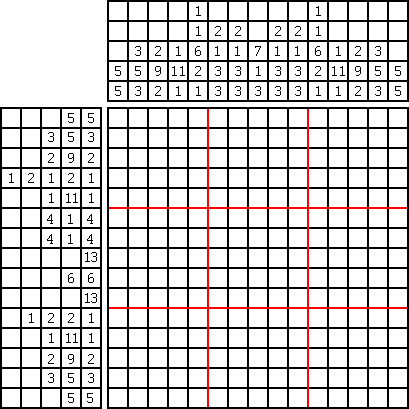
\includegraphics[scale=0.5]{PaintbyNumberExample.png}
	\label{figure:grille_initialisation}
\end{figure}\bigbreak
Avant d’expliquer les règles détaillées, voici une explication des différentes grilles~:\medbreak
\begin{itemize}[label=$\square$]
	\item la grille de jeu correspond à la grille centrale (figure \ref{figure:grille_initialisation})~;
	\item la grille périphérique verticale correspond à la grille située à gauche de la grille principale~;
	\item la grille périphérique horizontale correspond à la grille située au dessus de la grille principale~;
	\item la grille solution correspond à la grille que doit trouver le joueur pour terminer le niveau. Elle n'est jamais affichée à l'écran.
\end{itemize}\bigbreak
La seule grille que le joueur peut modifier est la grille de jeu. Le but de ce dernier est de la remplir en changeant la couleur de ses cases bu blanc au noir pour représenter le motif de la grille solution.
\begin{figure}[!h]
	\centering
	\caption[Comparaison solution et grille de jeu]{À gauche, le motif de la grille solution, à droite la grille de jeu remplie (source~: \href{https://commons.wikimedia.org/wiki/File:Picross_DS_Mini-Game.png}{Wikipédia})}\medbreak
	
\includegraphics{PicrossDSMini-Game.png}
	\label{figure:comparaison_grilles}
\end{figure}\bigbreak
Les grilles périphériques contiennent chacune des nombres. Ces nombres sont la représentation de la grille solution sous forme numérique. En effet, un nombre présent dans une colonne de la grille périphérique horizontale détermine un groupe de cases noires successives dans la colonne correspondante de la grille solution. Il peut y avoir plusieurs nombres dans une même rangée, et cela signifie qu’il y a donc plusieurs groupes de cases séparés d’au moins une case dans cette rangée. Le fonctionnement de la grille périphérique verticale est le même, à la différence près qu'elle renseigne les groupes de cases pour les lignes. Ainsi, avec toutes ces données présentes dans les grilles périphériques, il est possible de trouver le motif solution en changeant les cases de la grille de jeu en noire. Si celle-ci correspond bien à tous les nombres présents dans les matrices périphériques, le joueur termine le niveau et passe au suivant. Si le joueur termine le dernier niveau, il gagne la partie.
\begin{figure}[!h]
	\centering
	\caption[Grille complétée correctement]{Une grille brillamment remplie par le joueur (source~: \href{https://en.wikipedia.org/wiki/Nonogram}{Wikipédia})}\medbreak
	
\includegraphics[scale=0.15]{Nonogram.png}
	\label{figure:nonogram}
\end{figure}
\newpage
\section*{\LARGE IV. Codage, méthode et outils}
\addcontentsline{toc}{section}{IV. \quad Codage, méthode et outils}
\label{section*:codage_methode_outils}
\section*{A \hspace*{0.3cm} SDL}
\addcontentsline{toc}{section}{A \hspace*{0.15cm} SDL}
\label{section:sdl}
Ce programme fonctionne sur deux plate-formes~: le terminal et l'interface graphique (gérée par SDL2.0). SDL est une bibliothèque graphique qui permet d’obtenir un affichage géométrique plutôt que totalement numérique. Dans le cas du Picross, celle-ci sert à~:\medbreak
\begin{itemize}[label=$\square$]
	\item afficher la structure des grilles~;
	\item avoir un bouton pour soumettre la grille de jeu à une vérification~;
	\item pouvoir changer l’état des cases seulement en cliquant sur celles-ci.
\end{itemize}
\begin{figure}[!h]
	\centering
	\caption[Capture d'écran de l'interface du projet]{Capture d'écran de l'interface du projet (source~: PC de Benjamin)}\medbreak
	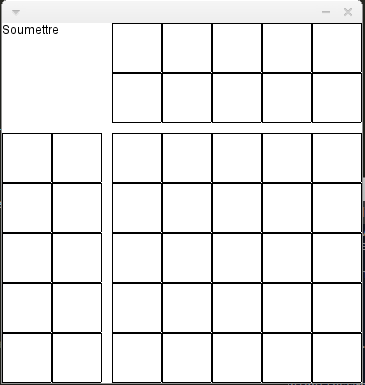
\includegraphics[scale=0.5]{sdl.png}\medbreak
	\label{figure:capture_ecran_sdl2}
\end{figure}\bigbreak
SDL est donc un bon moyen permettant au joueur d’avoir une expérience de jeu plus confortable et intuitif qu'avec un terminal. Néanmoins, la bibliothèque SDL seule dans le cas du Picross n’apporte que la structure graphique des matrices et le remplissage coloré des cases changées par l’utilisateur. Or, dans ce cas, il manque deux fonctionnalités essentielles~:\medbreak
\begin{itemize}[label=$\square$]
	\item le remplissage des grilles périphériques avec des nombres~;
	\item le bouton de validation de la réponse du joueur.
\end{itemize}\bigbreak
Pour accomplir ces attentes, la version graphique du Picross demande deux librairies supplémentaires~: \og SDL2\_ttf \fg{} et \og SDL2\_image \fg{}. Quant au reste du fonctionnement général, les fonctions utilisées pour la version \og terminal \fg{} sont reprises pour la version graphique.\medbreak
Ainsi, le code observé est sensiblement le même, hormis le fait qu’il faut initialiser, afficher, rafraîchir et détruire la fenêtre qui contient le jeu. En ce qui concerne la taille de la fenêtre d’affichage, elle est de taille unique en fonction de la dimension de la grille principale et est non-redimensionnable par le joueur. La taille d’une case est pensée pour qu’un nombre à deux chiffres puisse y être inséré, mais pas pour un nombre à trois chiffre. Chaque rangée des grilles périphériques est alignée avec la bonne colonne - ou ligne - de la grille de jeu. Enfin, le joueur peut décider d’arrêter lui-même sa partie en fermant la fenêtre avec la croix du menu de la fenêtre.
\section*{B \hspace*{0.3cm} Programmation modulaire}
\addcontentsline{toc}{section}{B \hspace*{0.15cm} Programmation modulaire}
\label{section:programmation_modulaire}
\subsection{Génération de matrices}
\begin{itemize}[label=$\square$]
	\item Création d'une matrice carré d'une taille n*n, n représentant la difficulté de complétion de la grille~;
	\item Création de deux matrices périphériques (horizontale en haut et verticale à gauche) en fonction de la matrice solution~;
	\item Lecture d'un fichier texte contenant les données nécessaires au remplissage des matrices périphérique, cette étape se realisera avec une fonction dediée à l'application
	des régles de remplissage des grilles.
\end{itemize}
\subsection{Modification des données lors d'une partie}
Voici les modifications assurées par la fonction \og \textbf{changerEtat([3 arguments])} \fg{}~:\medbreak
\begin{itemize}[label=$\square$]
	\item Au moment où le joueur se décide de cocher une case, la case vide recevra la valeur \og 1 \fg{} d'où \og 1 \fg{} représente une case remplie~;
	\item Si le joueur se décide de décocher une case déjà cochée, celle-ci recevra la valeur \og 2 \fg{} d'où \og 2 \fg{} représentera en graphique une croix (X)~;
	\item Décocher une croix permettra à la case de retrouver son statut initial (0).
\end{itemize}
\newpage
\section*{\LARGE V. \hspace*{0.05cm} Résultats et conclusion}
\addcontentsline{toc}{section}{V. \quad Résultats et conclusion}
\label{section*:resultats_conclusion}
Dans ce rapport, nous avons expliqué d’une manière générale les étapes de développement du jeu. Nous avons spécifié les besoins puis nous avons proposé une solution.\bigbreak
Voici une liste des différentes problèmes que nous avons pu détecter sans pouvoir leur trouver une solution viable~:\medbreak
\begin{itemize}[label=$\blacksquare$]
	\item la fonction \textbf{lecture\_fic([5 arguments])} ne gère pas toujours les sauts de lignes entre chaque ligne de nombres, ce qui restreint le format trouvé.
\end{itemize}\bigbreak
De même, en-dehors des fonctions, la gestion du groupe (attribution des rôles et des fonctions à coder) n'a pas été un franc succès pendant un long moment et cela a conduit à un manque de temps et de cohérence pour intégrer les fonctions attendues dans les fichiers exécutables. Néanmoins, voici quelques idées d'améliorations possibles trouvées pendant le semestre~:\medbreak
\begin{itemize}[label=$\square$]
	\item une interface graphique convenable~;
	\item un affichage dynamique en fonction de la complétion de chaque rangée (grisage automatique)~;
	\item l'ajout d'un timer pendant une partie~;
	\item l'ajout d'un système de score.
\end{itemize}\bigbreak
Ce projet nous a permis de nous familiariser avec certains outils informatiques vu en cours. Enfin, nous aurions pu réaliser toutes les améliorations citées ci-dessus, mais le temps nous a manqué.
\end{document}